\begin{figure}[t]
\begin{center}
\begin{small}
\begin{sc}
\begin{subfigure}[b]{.23\textwidth}
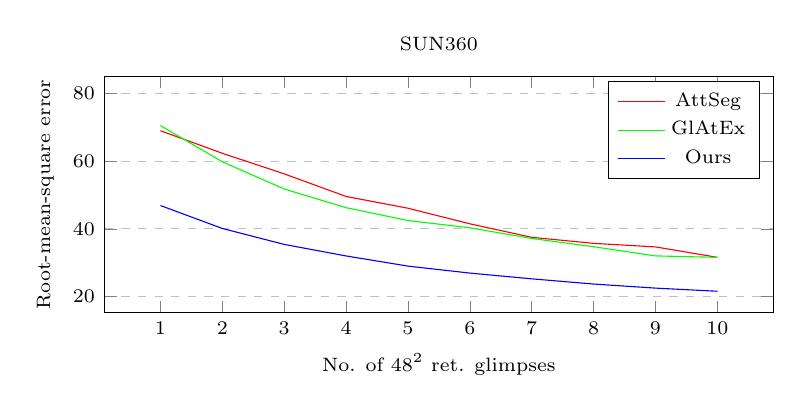
\begin{tikzpicture}
\tikzstyle{every node}=[font=\scriptsize]
\begin{axis}[
    title={SUN360},
    xlabel={No. of $48^2$ ret. glimpses},
    ylabel={Root-mean-square error},
    xtick={1,2,3,4,5,6,7,8,9,10},
    ymajorgrids=true,
    grid style=dashed,
    scale only axis,
    height=3cm,
    ymax=85,
    width=.7\textwidth
]
\addplot[color=red]
    coordinates {
    (1,68.99)(2,62.32)(3,56.24)(4,49.57)(5,46.09)(6,41.49)(7,37.49)(8,35.71)(9,34.66)(10,31.58)
    };
\addlegendentry{AttSeg}
\addplot[color=green]
    coordinates {
    (1,70.50)(2,59.81)(3,51.77)(4,46.25)(5,42.45)(6,40.31)(7,37.16)(8,34.72)(9,32.00)(10,31.58)
    };
\addlegendentry{GlAtEx}
\addplot[color=blue]
    coordinates {
    (1,46.89)(2,40.11)(3,35.40)(4,31.99)(5,28.99)(6,26.93)(7,25.23)(8,23.69)(9,22.49)(10,21.56)
    };
\addlegendentry{Ours}
\end{axis}
\end{tikzpicture}
\end{subfigure}
\begin{subfigure}[b]{.23\textwidth}
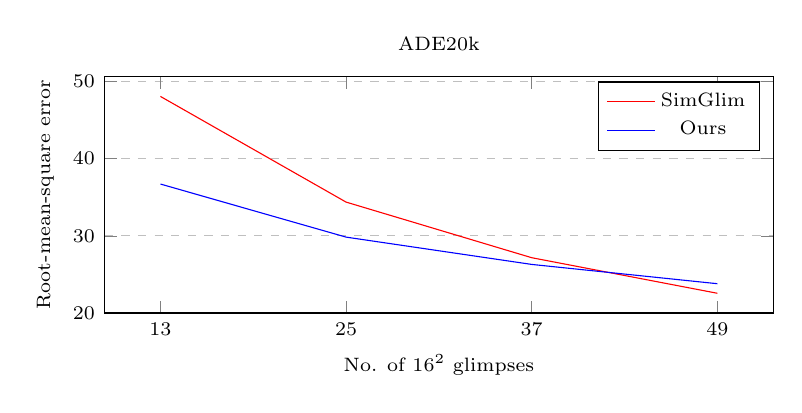
\begin{tikzpicture}
\tikzstyle{every node}=[font=\scriptsize]
\begin{axis}[
    title={ADE20k},
    xlabel={No. of $16^2$ glimpses},
    ylabel={Root-mean-square error},
    xtick={13,25,37,49},
    ymajorgrids=true,
    grid style=dashed,
    scale only axis,
    height=3cm,
    width=.7\textwidth
]
\addplot[color=red]
    coordinates {
    (13,48.08)(25,34.38)(37,27.17)(49,22.56)
    };
\addlegendentry{SimGlim}
\addplot[color=blue]
    coordinates {
    (13,36.72)(25,29.84)(37,26.30)(49,23.80)
    };
\addlegendentry{Ours}
\end{axis}
\end{tikzpicture}
\end{subfigure}
\end{sc}
\end{small}
\end{center}

\caption{\textbf{Comparative reconstruction results in regards to glimpse selection step}: Figures present the effect of the number of glimpses on the reconstruction task. On the left, we compare our model against AttSeg~\protect\cite{seifi2020segment} and GlAtEx~\protect\cite{seifi2021glimpse} on the SUN360 dataset in $48^2$ retinal glimpse scenario. On the right, we compare our model against SimGlim~\protect\cite{Jha2023WACV} on ADE20K dataset in $16^2$ non-retinal glimpse task. Our solution outperforms competitive solutions when only a small amount of the image is available.}
\label{fig:nglimpses}
\end{figure}